\documentclass[10pt]{article}

\usepackage{blindtext}
\usepackage{etex}
\usepackage{makeidx}  % allows for indexgeneration
\usepackage{mathtools} %
\usepackage{booktabs} %
\usepackage{verbatim} %
\usepackage{graphicx}
\usepackage{amsmath}
\usepackage{amssymb}
\usepackage{amsthm}
\usepackage{xspace}
\usepackage{natbib}
\usepackage{pifont}%
\usepackage{tikz}
\usepackage{relsize}
\usepackage{multirow}
\usepackage{textcomp}
\usepackage{comment}
\usepackage{url}
\usepackage{float}
%\usepackage{algorithmic}
\usepackage{algorithm}
\usepackage{algpseudocode}
%\usepackage[vlined]{algorithm2e}
\usepackage{subfig}
\usepackage{framed}
\usepackage{empheq}

\newcommand{\cmark}{\ding{51}}%
\newcommand{\xmark}{\ding{55}}%
\newcommand{\vectornorm}[1]{\left|\left|#1\right|\right|}
\newcommand{\argmin}{\operatornamewithlimits{argmin}}
\newcommand{\argmax}{\operatornamewithlimits{argmax}}

\algdef{SE}[DOWHILE]{Do}{doWhile}{\algorithmicdo}[1]{\algorithmicwhile\ #1}%

\newtheorem{problem}{Problem}

\begin{document}

\title{Efficient Selection of Optimal Time Points Over Biological Time-Series Data}
\date{}

\maketitle

\section{Methods}

\subsection{Problem statement}
Our goal is to identify a (small) subset of time points that can be
used to accurately reconstruct the expression trajectory for {\em
all} genes or other molecules being profiled. We assume that we can
efficiently and cheaply obtain a dense sample for the expression of
a very small subset of representative genes (here we use nanostring
to profile less than $0.5\%$ of all genes) and attempt to use this
subset to determine optimal sampling points for the entire set of
genes.

Formally, let $G$ be the set of genes we have profiled in our dense
sample, $T = \{t_{1}, t_{2}, \ldots, t_{T}\}$ be the set of all
sampled time points. We assume that for each time point we have $R$
repeats for all genes. We denote by $e_{gt}^{r}$ be the expression
value for gene $g \in G$ at time $t \in T$ in the $r$'th repeat for
that time point. We define $D_{g} = \{e_{gt}^{r}\,,\, t \in T, r \in
R$ as the complete data for gene $g$ over all replicates and time
points $T$.

To constrain the set of points we select we assume that we have a
predefined budget $k$ for the maximum number of time points we can
sample in the complete experiment (i.e. for profiling all genes, miRNAs, epigenetic marks etc. using high throughput seq
experiments). We are interested in selecting $k$ time points from
$T$ which, when using only the data collected at these $k$ points,
minimizes the prediction error for the expression values of the
unused points. To evaluate such a selection, we use the selected
values to obtain a smoothing splines~\cite{deboor, bar2003,
wahba1990} function for each gene and compare the predicted values
based on the spline to the measured value for the non-selected
points to determine the error. In our problem, $t_{1}$ and $t_{T}$
define the first and end points, so they are always selected. The
rest of the points are selected to maximize the following
objective~\ref{prob:prob1}:
%
\begin{problem}\label{prob:prob1}
Given $D_{g}$ for genes $g \in G$, the number of desired time points
$k$ identify a subset of $k-2$ time points in $T \setminus \{t_{1},
t_{T}\}$ which minimizes the prediction error for the expression
values of all genes in the remaining time points.
\end{problem}


\subsection{Spline assignments}

Before discussing the actual procedure we use to select the set of
time points, we discuss the method we use to assign splines based on
a selected subset of point $k$ for each gene. There are two issues
that needs to be resolved when assigning such smoothing splines: 1.
The number of knots (control points) and 2. their spacing. Past
approaches for using splines to model time series gene expression
data have usually used the same number of control points for all
genes regardless of their trajectories~\cite{bar2012, singh2005} and mostly employed uniform
knot placements. However, since our method needs to be able to adapt
to any size of $k$ as defined above, we select them indirectly through
regularization parameter of the fitted smoothing spline where number
of knots will be increased until the smoothing condition is
satisfied. In contrast to the existing methods, we also select knots when fitting a smoothing spline.

\subsection{Iterative process to select points}\label{sec:mainalgo}

Because of the highly combinatorial nature of the time points, selection problem we rely on a greedy iterative process to select
the optimal points as shown in Algorithm~\ref{alg:algo}.
%Figure ~\ref{fig:algo}.

There are three key steps in this algorithm which we discuss in
detail below.

\begin{itemize}
\item {\em Selecting the initial set of points:} When using an iterative algorithm to solve non convex problems with several local minima,
a key issue is the appropriate selection of the initial solution
set~\cite{kmeans, mixture}. We have tested a number
of methods for performing such initializations. The simplest method
we tried is to uniformly select a subset of the points (so if
$k=T/4$ we use each 4th point). Another method we tested is to partition the set
of all time points $T$ into $k-1$ intervals of almost equal size by
dynamic programming. Then, it uses $k$ interval boundaries including
$t_{1}$ and $t_{T}$ as initial solution. Finally, we tested a
method that relies on the changes between consecutive time points to
select the most important ones for our initial set. Specifically,
for this we sort all points except $t_{1}$ and $t_{T}$ by average
absolute difference with respect to its predecessor time points by
computing:
%
\begin{equation}
m_{t_{i}} = \frac{\sum_{g \in G} \sum_{d \in D}\,|e_{g t_{i-1}} -
e_{g t_{i}}|}{2 \sum_{g \in G} |D_{g}|}
\end{equation}
where $g t_{i}$ is the average or median expression for gene $g$ at
time $t$. We then select the $k-2$ points with maximum $m_{t_{i}}$
as the initial solution.

\item After selecting the initial set, we begin the iterative process of refining the subset of selected points.
In this step we repeat the following analysis in each iteration. We
exhaustively remove all points from the existing solution (one at a
time) and replace it with all points that were not in the selected
set (again, one at a time). For each pair of such point, we compute
the error resulting from the change (using the splines computed
based on the current set of points evaluated on the left out time
points), and determine if the new point reduces the error or not.
Formally, let $C_n$ be set of points for iteration $n$ We are
interested in finding a point pair $(t_{a} \in C_n, t_{b} \in T
\setminus C_n)$
which minimizes the following error for the next iteration $C_{n+} =
C_n \setminus \{t_{a}\} \cup \{t_{b}\}$:
%
\begin{equation}
\textit{error} = \frac{\sum_{g \in G} \sum_{d \in D}\, \sum_{t \in
    T \setminus C_{n+1}}|\hat{e}_{gt} - e_{gt}^{d}|}{\sum_{g \in G}
  \sum_{d \in D} \sum_{t \in
    T \setminus C_{n}} |\hat{e}_{gt} - e_{gt}^{d}|}
\end{equation}
%
where $\hat{e}_{gt}$ is our spline based estimate of the expression
of gene $g$ at time $t$. If there are pairs which leads to an error
of less than $1$ in the above function, we select the best (lowest
error) and continue the iterative process. Otherwise we terminate
the process and output $C_n$ as the optimal solution. Note that this
greedy process is guaranteed to converge to a (local) minima since
the number of time points is finite.

% \begin{figure}
% \centering
% 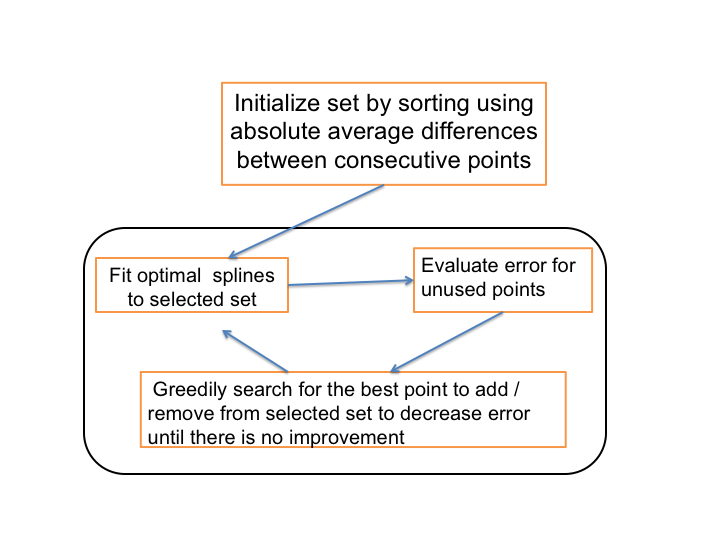
\includegraphics[scale=0.4]{algo.png}
% \caption{Summary of our Method}
% \label{fig:algo}
% \end{figure}

\begin{algorithm}
\caption{Iterative $k$-point selection}
\label{alg:algo}
\begin{algorithmic}[1]
\Procedure{Iterative\textendash Selection}{}
\State $C_{0} = $ select initial $k$ time points by absolute value sorting
\State $e_{0} = $ error of remaining points by fitting splines to $C_{0}$
\State $i=0$
\Do
\For{each pair $(a, b) \in (T - C_{i}) \times C_{i}$}
\State $C^{*} = C_{i} \cup \{ a \} \setminus \{b\}$
\State $e^{*} = $ estimate error by fitting smoothing spline to $C^{*}$
\If{$e^{*} < e_{i}$}
\State $C_{i+1} = C^{*}$
\State $e_{i+1} = e^{*}$
\EndIf
\State $i = i+1$
\EndFor
\doWhile{$e_{i+1} < e_{i}$}
\State Output $C_{i+1}$ and $e_{i+1}$
\EndProcedure
\end{algorithmic}
\end{algorithm}

\item Third key step of our approach is fitting smoothing spline to gene independently for selected subset of time points. Smoothing
  splines are capable of modeling arbitrary nonlinear shapes as well
  they do not have the problems seen in other polynomial fitting
  methods such as Runge's phenomenon. Smoothing splines perform quite well in preventing overfitting~\cite{wahba1990}. Let
  $R = \{(t, y_{t}),\, t \in C\}$, and $\mu$ be the spline we are interested in fitting, smoothing spline
  can be found by the following optimization problem which minimizes
  regularized squared error:
%
\begin{equation}
min \sum_{(t, y_{t}) \in R} \,(y_{t} - \mu(t))^{2} + \lambda \int_{0}^{T_{max}} (\mu^{''}(x))^{2}
\end{equation}
%
where $\lambda$ is the regularization parameter which prevents overfitting. We have estimated regularization parameter by leave one
out cross validation in our experiments. $\lambda$ also affects the number of knots selected.

\end{itemize}


\subsection{Individual vs. Cluster based Evaluation}\label{sec:clusteval}

In section~\ref{sec:mainalgo}, we assume that error of each gene has same contribution to the overall error. However, this assumption ignores the
fact that expression of genes are correlated with the expression of other genes. To take the
correlation between genes into account, we have also performed cluster
based evaluation of genes where we analyzed the error by weighting each gene in terms of inverse of the numbers of
genes in the cluster it belongs. This scheme ensures that each cluster
contributes equally to the resulting error rather than each gene. We find clusters by k-means
clustering algorithm over time series-data as well as over a vector of
randomly sampled time points on fitted spline~\cite{bishop2006}. We use Bayesian Information Criterion~(BIC) to
determine the optimal number of clusters~\cite{bic}.

\section{Results}


We developed a method to select a subset of $k$ time points from an
initial larger set of $n$ points such that the selected subset
provides an accurate, yet compact, representation of the temporal
trajectory.  The method utilizes splines to represent temporal
profiles and implements a cross validation strategy to evaluate
potential sets of points. Following initialization (which is based
on the expression values) we employ a greedy search procedure adds
and removes points until a local maxima is reached. The resulting
set is then used for the larger genomic and epigenetic experiments.

To test this method and to demonstrate its ability to reduce time,
costs and samples while still providing accurate description of the
temporal profiles we focused on a experiments related to lung
development in mice. We initially selected a subset of genes 134
genes that were previously determined to be involved in lung
development (Methods) and have profiled them using a NanoString
array at a high sampling rate.  Specifically, we profiled these
genes at 40 {\em I thought we excluded 9.5 and 10.5 due to their
variability, no?} time points between day 0.5 and day 28 with 3 to 5
repeats for each time point (Methods). Data was normalized using
{\em what normalization method was used?}.

\subsection{Using mRNA expression values to select a subset of time points}\label{sec:findsubset}

%identified points


%(+ additional anchor points of E16.5 and E18.5 for other analyses)

%performance comparison
We tested the performance of our method by using it to select
subsets of size {\em what's the lowest number, 3}? to 25 time
points. To determine the accuracy of the reconstructed profiles
using the selected points we computed the average error for points
that were not used by the method (Methods). The results are
presented in Figure ~\ref{fig:errplots} which also plots a
comparison between the performance of our method and two baseline
approaches: a random selection of points and uniform sampling {\em
can you add uniform here?} which is often used in such experiments
{\em reference}. We have also compared the performance of the
different strategies to initialize the set of points and to perform
the search. Finally, the figure includes a comparison between the
performance of each of these strategies and the noise in the data
{\em can you add this as a line} (computed based on the repeat
information) which is the theoretical limit for the performance of
any profile reconstruction method. As can be seen in the Figure, we
find significant performance improvement over randomly selected
points as in Figure~\ref{fig:errplots} in terms of mean squared
error. Sorting initial points by absolute values further improves
the performance highlighting the importance of initialization when
searching large combinatorial spaces.

As the number of points used by the method increases the performance
leads to results that are very close to the error represented by
noise in the data even when only using half the points.

\begin{figure}
\centering
\includegraphics[scale=0.2]{{../newdata/perform}.png}
\caption{Performance of our method by increasing number of selected points}
\label{fig:errplots}
\end{figure}

Figure~\ref{fig:centplots} presents the reconstructed and measured
expression values for a few genes using $13$ time points. Note that
even though each of these genes had a different trajectory and
different inflection points, the selected set of points enables our
method to fit all of these pretty well.

\begin{figure}
\begin{minipage}{1.0\textwidth}
\subfloat[PDGFRA]{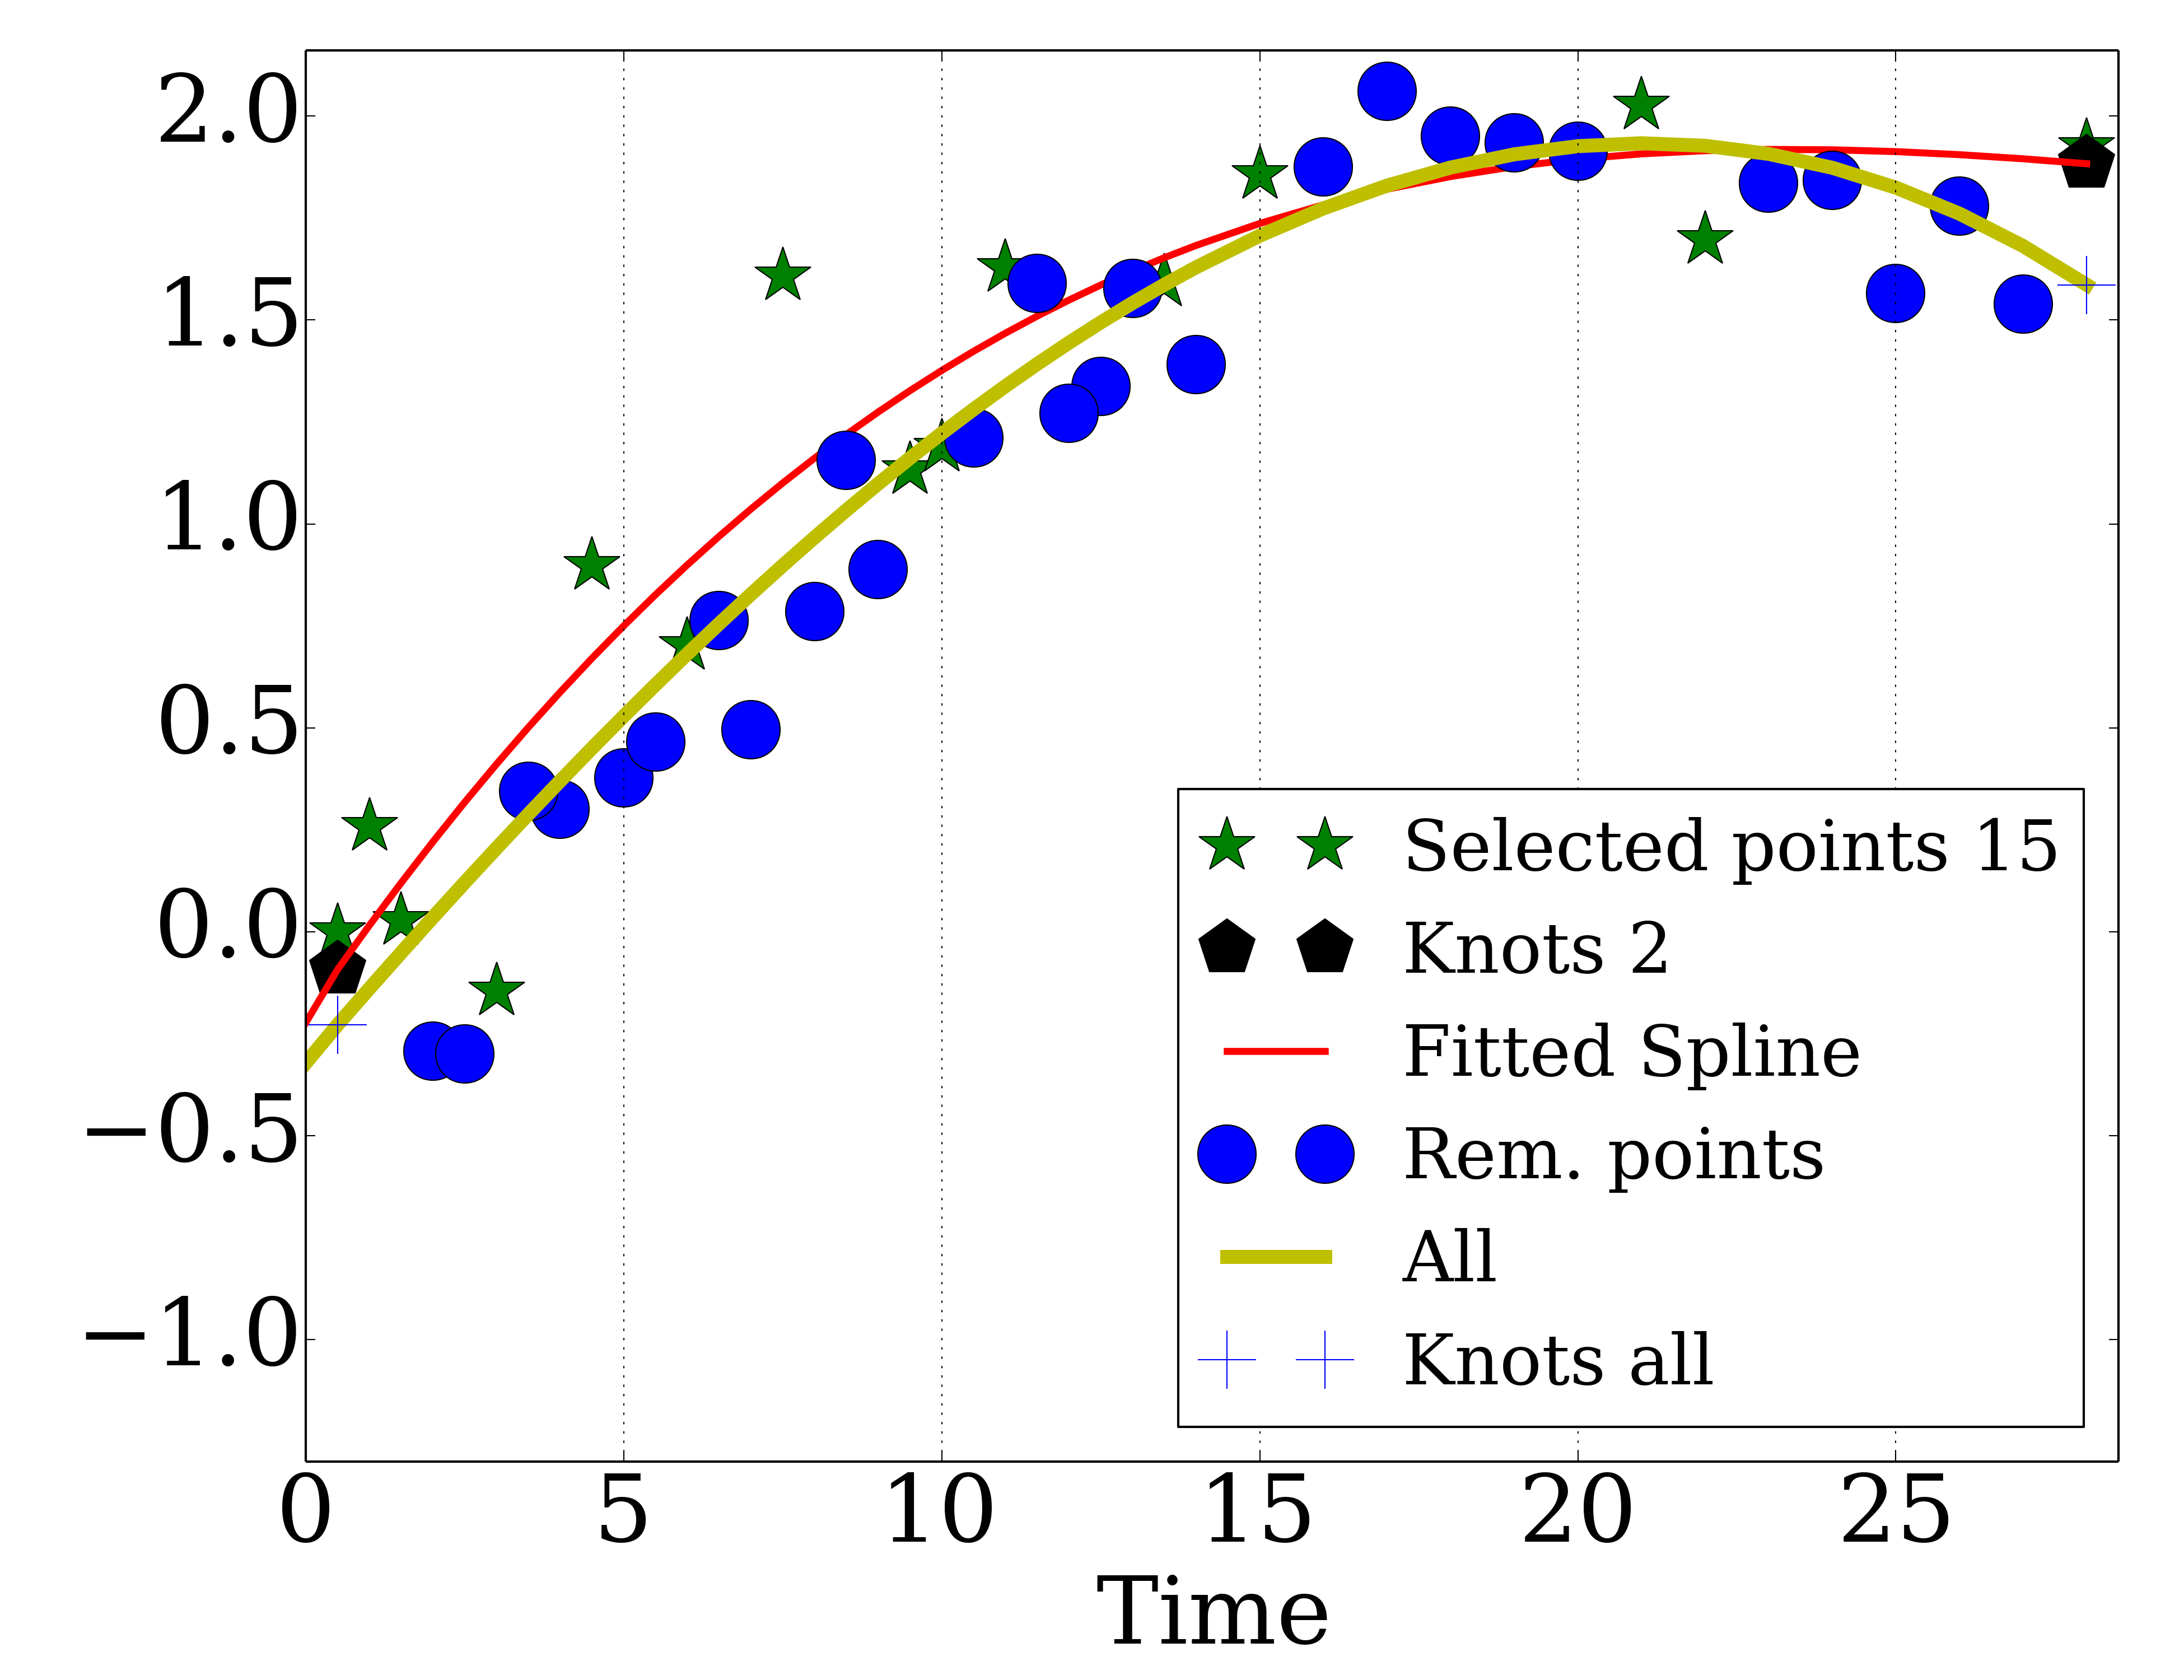
\includegraphics[scale=0.12]{{../newdata/PDGFRA_15_all}.png}}
\hfill
\subfloat[ELN]{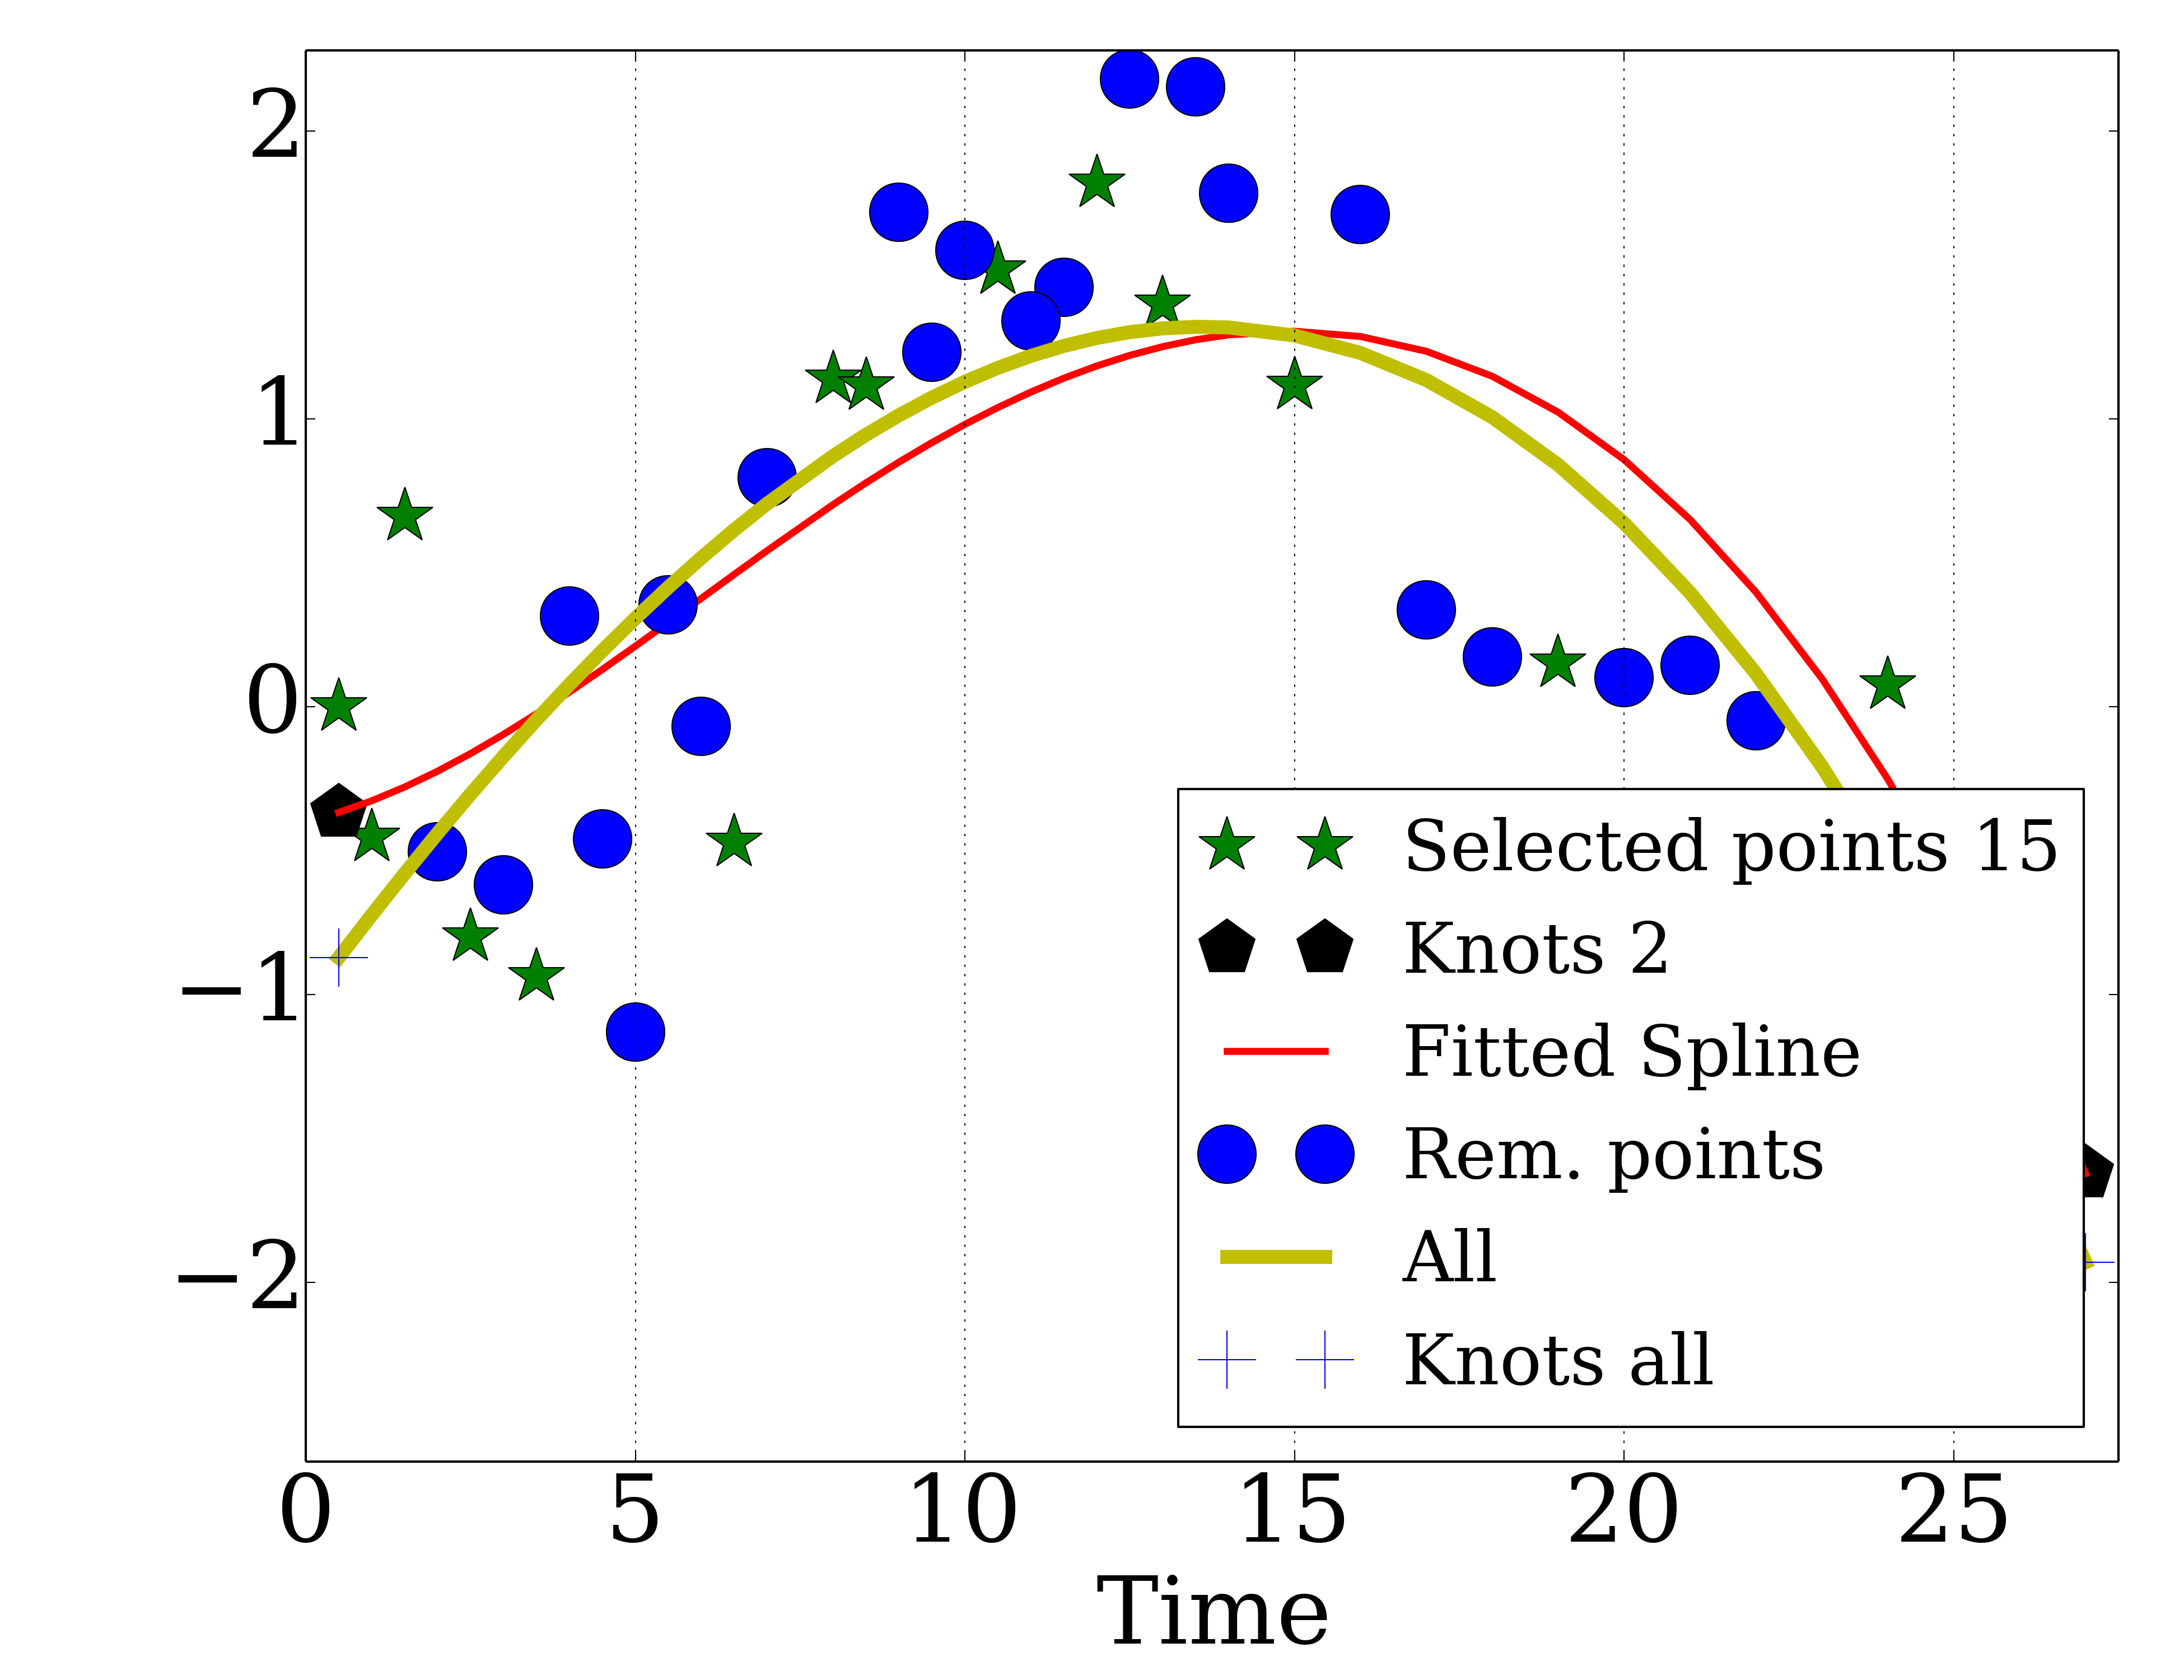
\includegraphics[scale=0.12]{{../newdata/splineplots15/Eln_15_all}.png}}
\hfill
\subfloat[INMT]{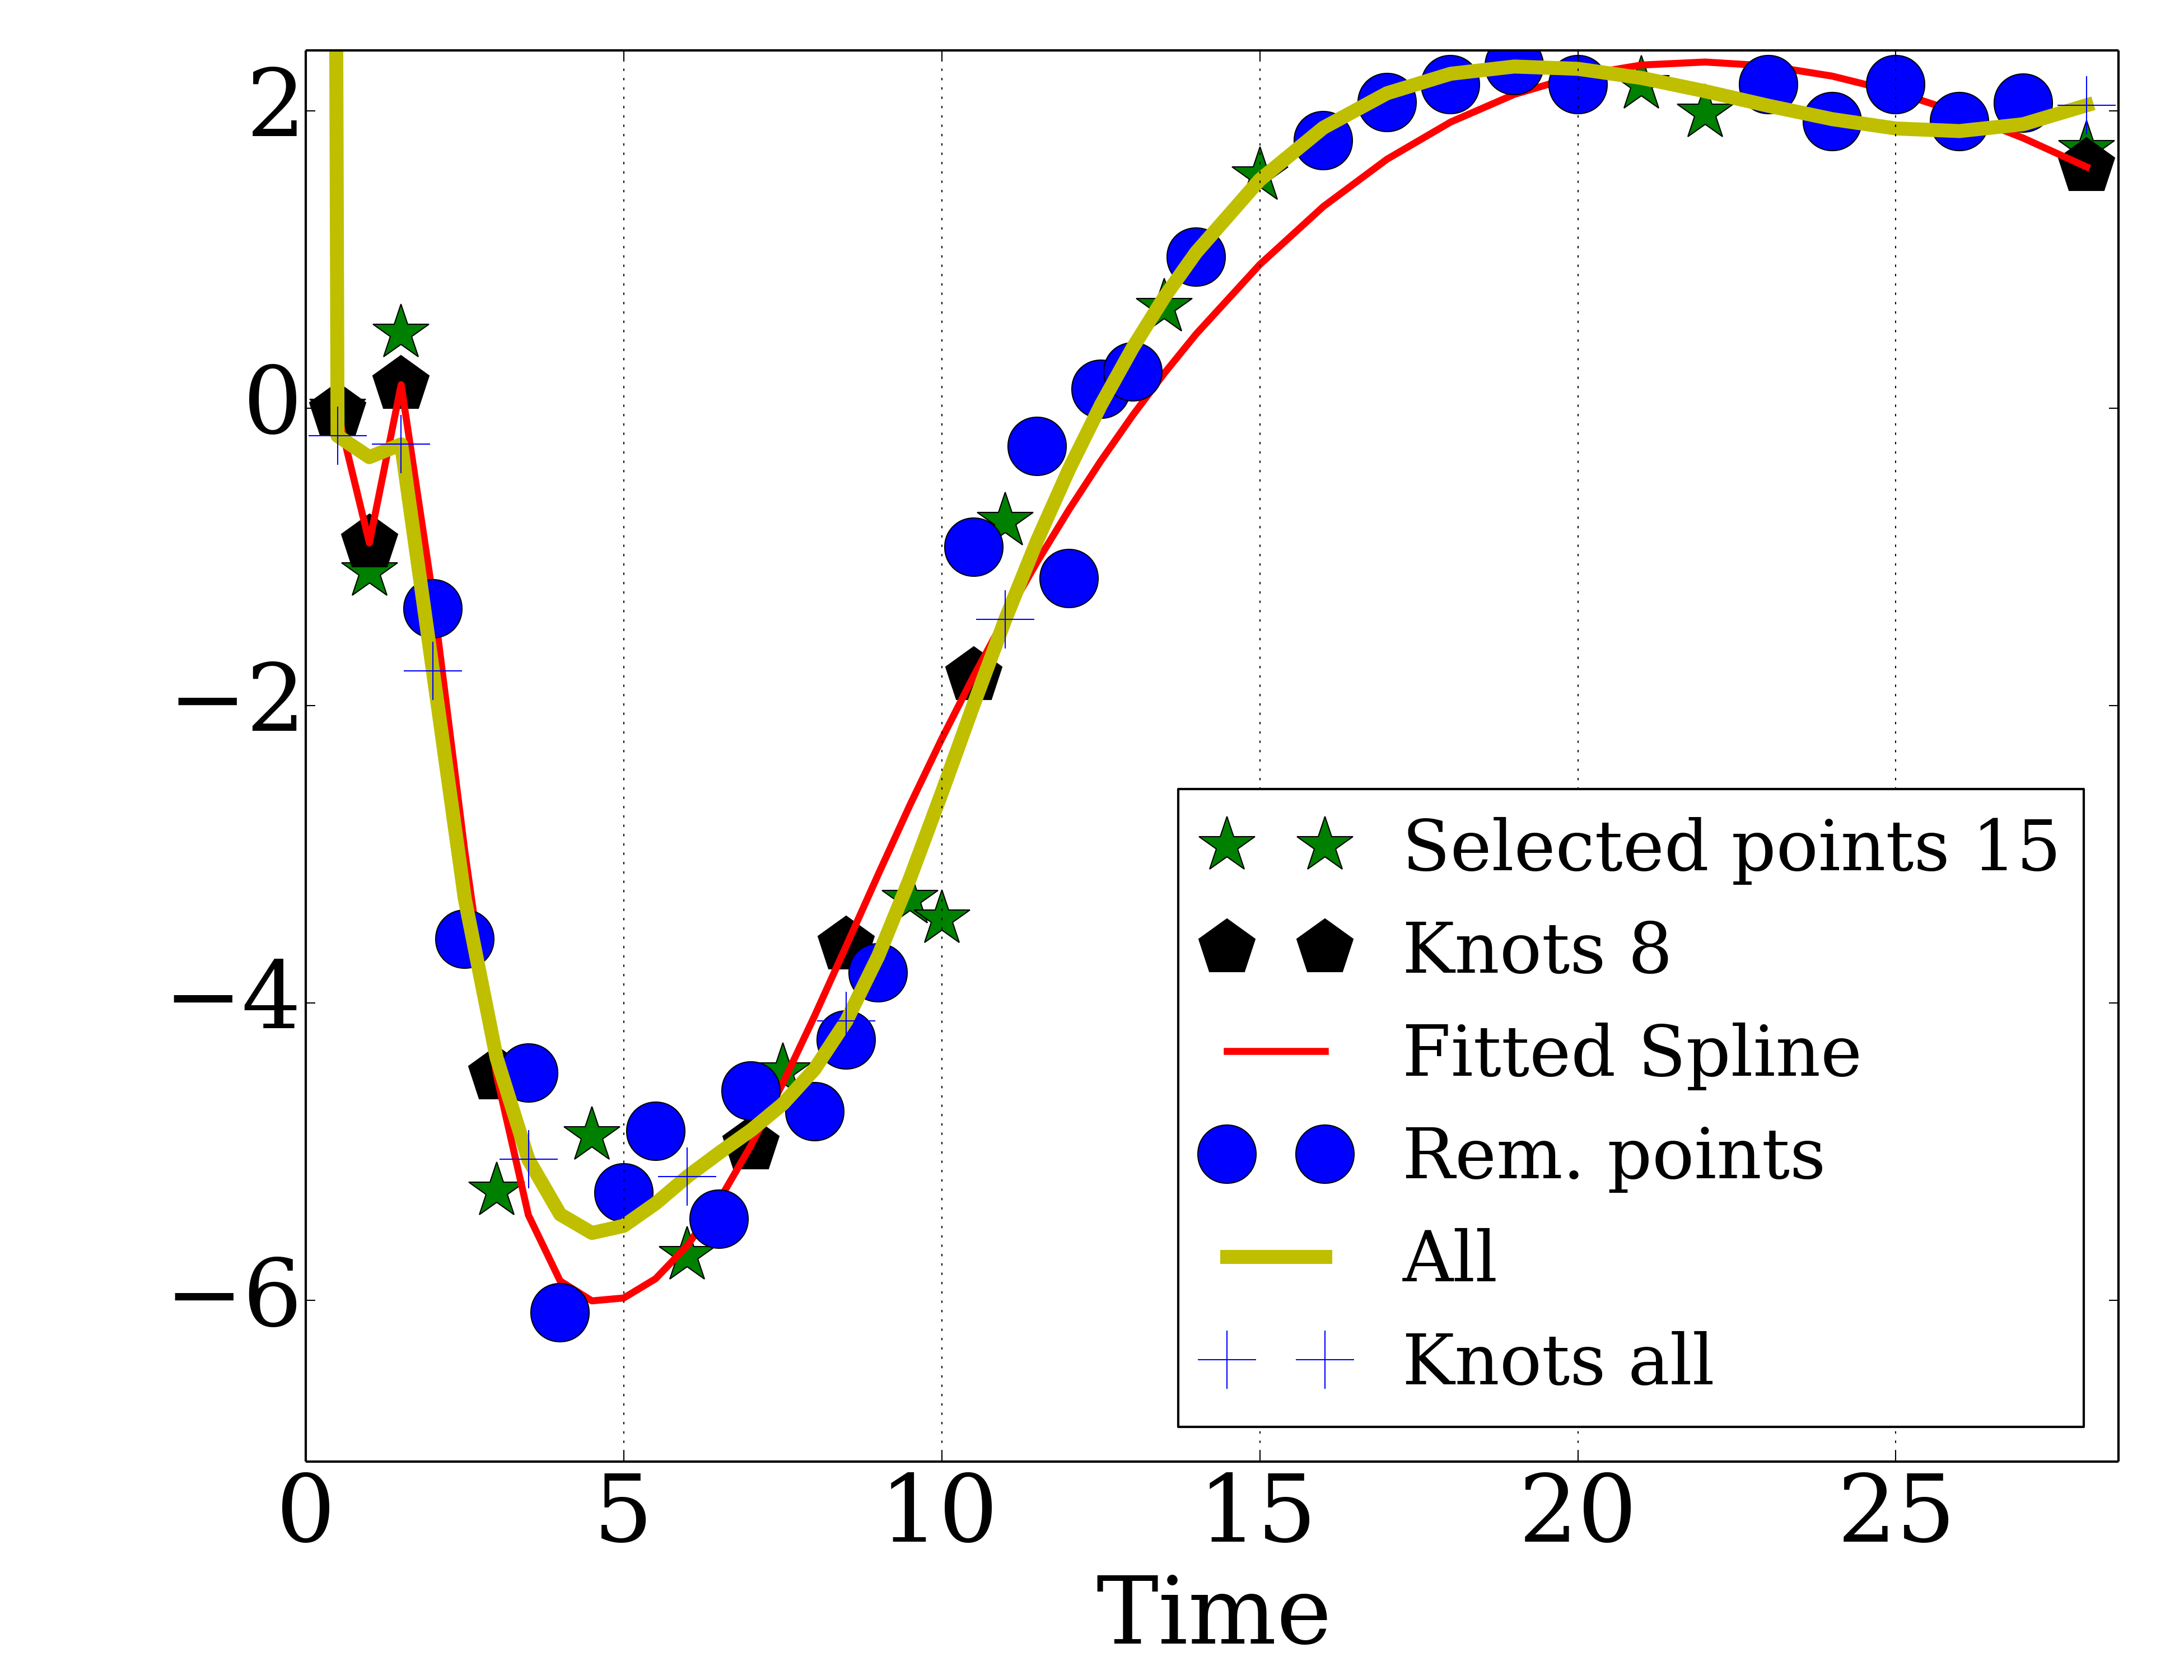
\includegraphics[scale=0.12]{{../newdata/splineplots15/INMT_15_all}.png}}
\hfill
\end{minipage}
\caption{Expression profiles over several genes a) PDGFRA, b) ELN, c) INMT}
\label{fig:centplots}
\end{figure}

{\em why do we need this: While our method can be used to select any
number of time points, to demonstrate its utility we have tested it
in the following setting. First we fixed a set of points (first and
last, which are required for any setting and day 7 which was
previously determined to be of importance to lung development, see
Supporting Results for other settings). In addition, we have asked
the method to further select 10 more points (for a total of 13). For
this setting the method selected the following points: w$0.5$,
$1.0$, $1.5$, $2.5$, $4$, $5$, $7$, $10$, $13.5$, $15$, $19$, $23$,
$28$. While we do not know the ground truth, the larger focus on the
earlier time points determined by the method (with 7 of the 13
points for the first 7 days) makes sense in this context as several
aspects of lung differentiation are determined in this early phases
{\em any reference here?}. The other 3 weeks were more or less
uniformly sampled by our method. This highlights the usefulness of
an unbiased approach to sampling time points rather than just
uniformly sampling through the time window.}

{\em what about cluster based results? Can you say something here
about them?}
\subsection{mRNA based sampling rates accurately  reconstruct miRNA expression profiles}\label{sec:mirnaexp}

To test the usefulness of our method for predicting the correct
sampling rates for other genomic datasets we next profiled mouse
miRNAs for the same developmental process {\em a few words here on
why miRNAs are important for lung development}. Unlike the mRNA
dataset, which utilized prior knowledge to profile less than 1\% of
all genes, the miRNA dataset profiled 600 miRNAs, more than 50\% of
known mouse miRNAs {\em check}. Thus, such data represents an
unbiased sample and can provide information on whether using one
type of genomic data can be helpful for determining rates for other
types. To test the usefulness of our approach we used the miRNA
expression values for the time points determined by the mRNA
analysis to reconstruct the complete trajectories for each miRNA.
The results are presented in Figure~\ref{fig:mirnaerrplots}. In
addition the comparison included in the mRNA figure, the miRNA
figure includes the optimal results for using miRNA data (as opposed
to mRNA data) to select the points {\em we need to add this}. As can
be seen, the points selected by the mRNA analysis leads to
reconstruction that is much better than when using random points
highlighting the relationship between the two datasets and the
abiliyt to use one to determine points for the other. Further,
performance using the mRNA set is very similar to the performence
using the miRNA data itself. For example, when using the $13$
selected mRNA points the average error is $0.3312$ whereas when
using the optimal points based on the miRNA data itself the error
 is $0.3042$. This serves as  a strong indication that mRNAs can serve as a general proxy for
selecting time points.

%Identified time points are effective across multiple experiments.
%The effectiveness of identified time points across experiments show the importance of xxx and yyy.
%We also analyze the similarity of miRNA optimal points to mRNA optimal
%points as in Figure~\ref{xxx}.

\begin{figure}
\centering
\includegraphics[scale=0.2]{{../mirnadata/perform}.png}
\caption{Performance analysis over miRNA dataset}
\label{fig:mirnaerrplots}
\end{figure}

\subsection{Detailed Analysis of miRNA Dataset}\label{sec:mirna}

 Detailed analysis of
miRNA dataset shows clustered expression profiles of miRNAs as in
Figure~\ref{fig:clustmirna}. We identified $8$ stable clusters by
k-means~\cite{kmeans} where number of clusters is selected by
Bayesian Information Criteria~\cite{bic}. We find clusters to change
more frequently than mRNA data since miRNA is noisier than mRNA
data. Identified clusters are also enriched for several Gene
Ontology biological processes~\cite{go}.

\begin{figure}[h]
\centering
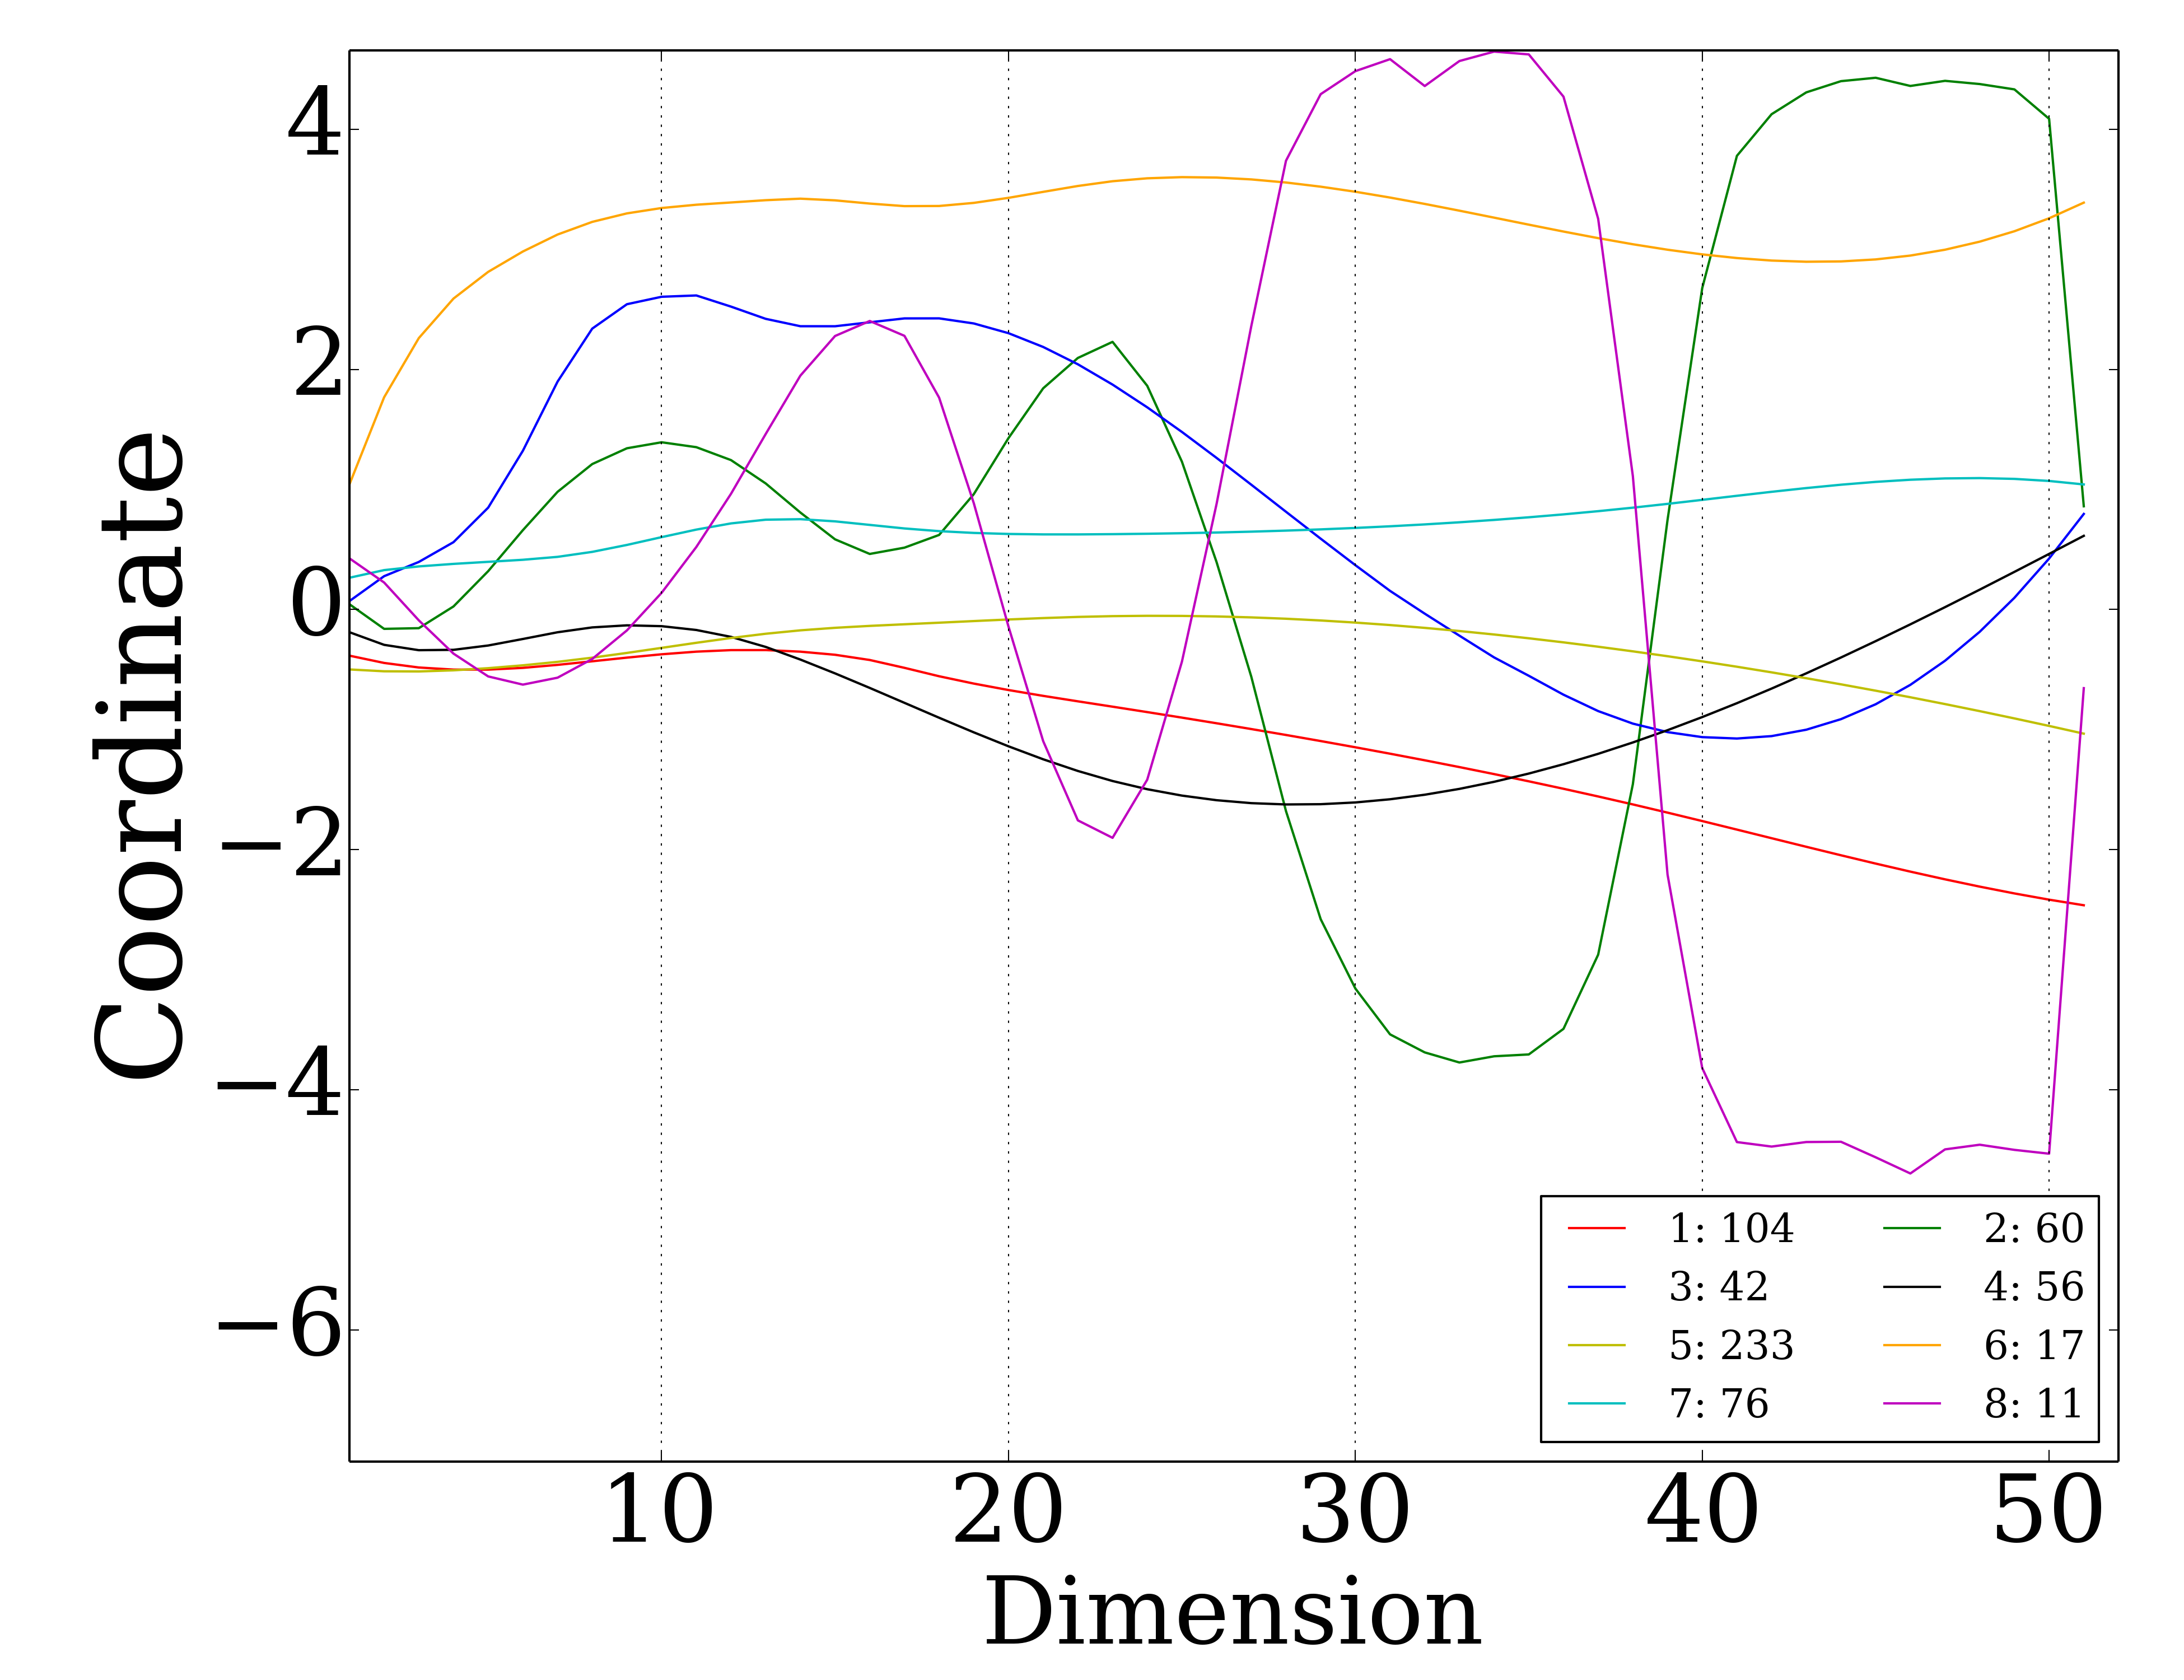
\includegraphics[scale=0.2]{{../mirnadata/centplot}.png}
\caption{$8$ stable clusters}
\label{fig:clustmirna}
\end{figure}


Figure~\ref{fig:mirnaplots_spec} presents a number of miRNAs that
are known to be regulating important developmental proteins. As can
be seen, using a subset of the points leads to accurate
reconstruction of their expression trajectories.

\begin{figure}[h]
\centering
\begin{minipage}{1.0\textwidth}
\subfloat[mmu-miR-100]{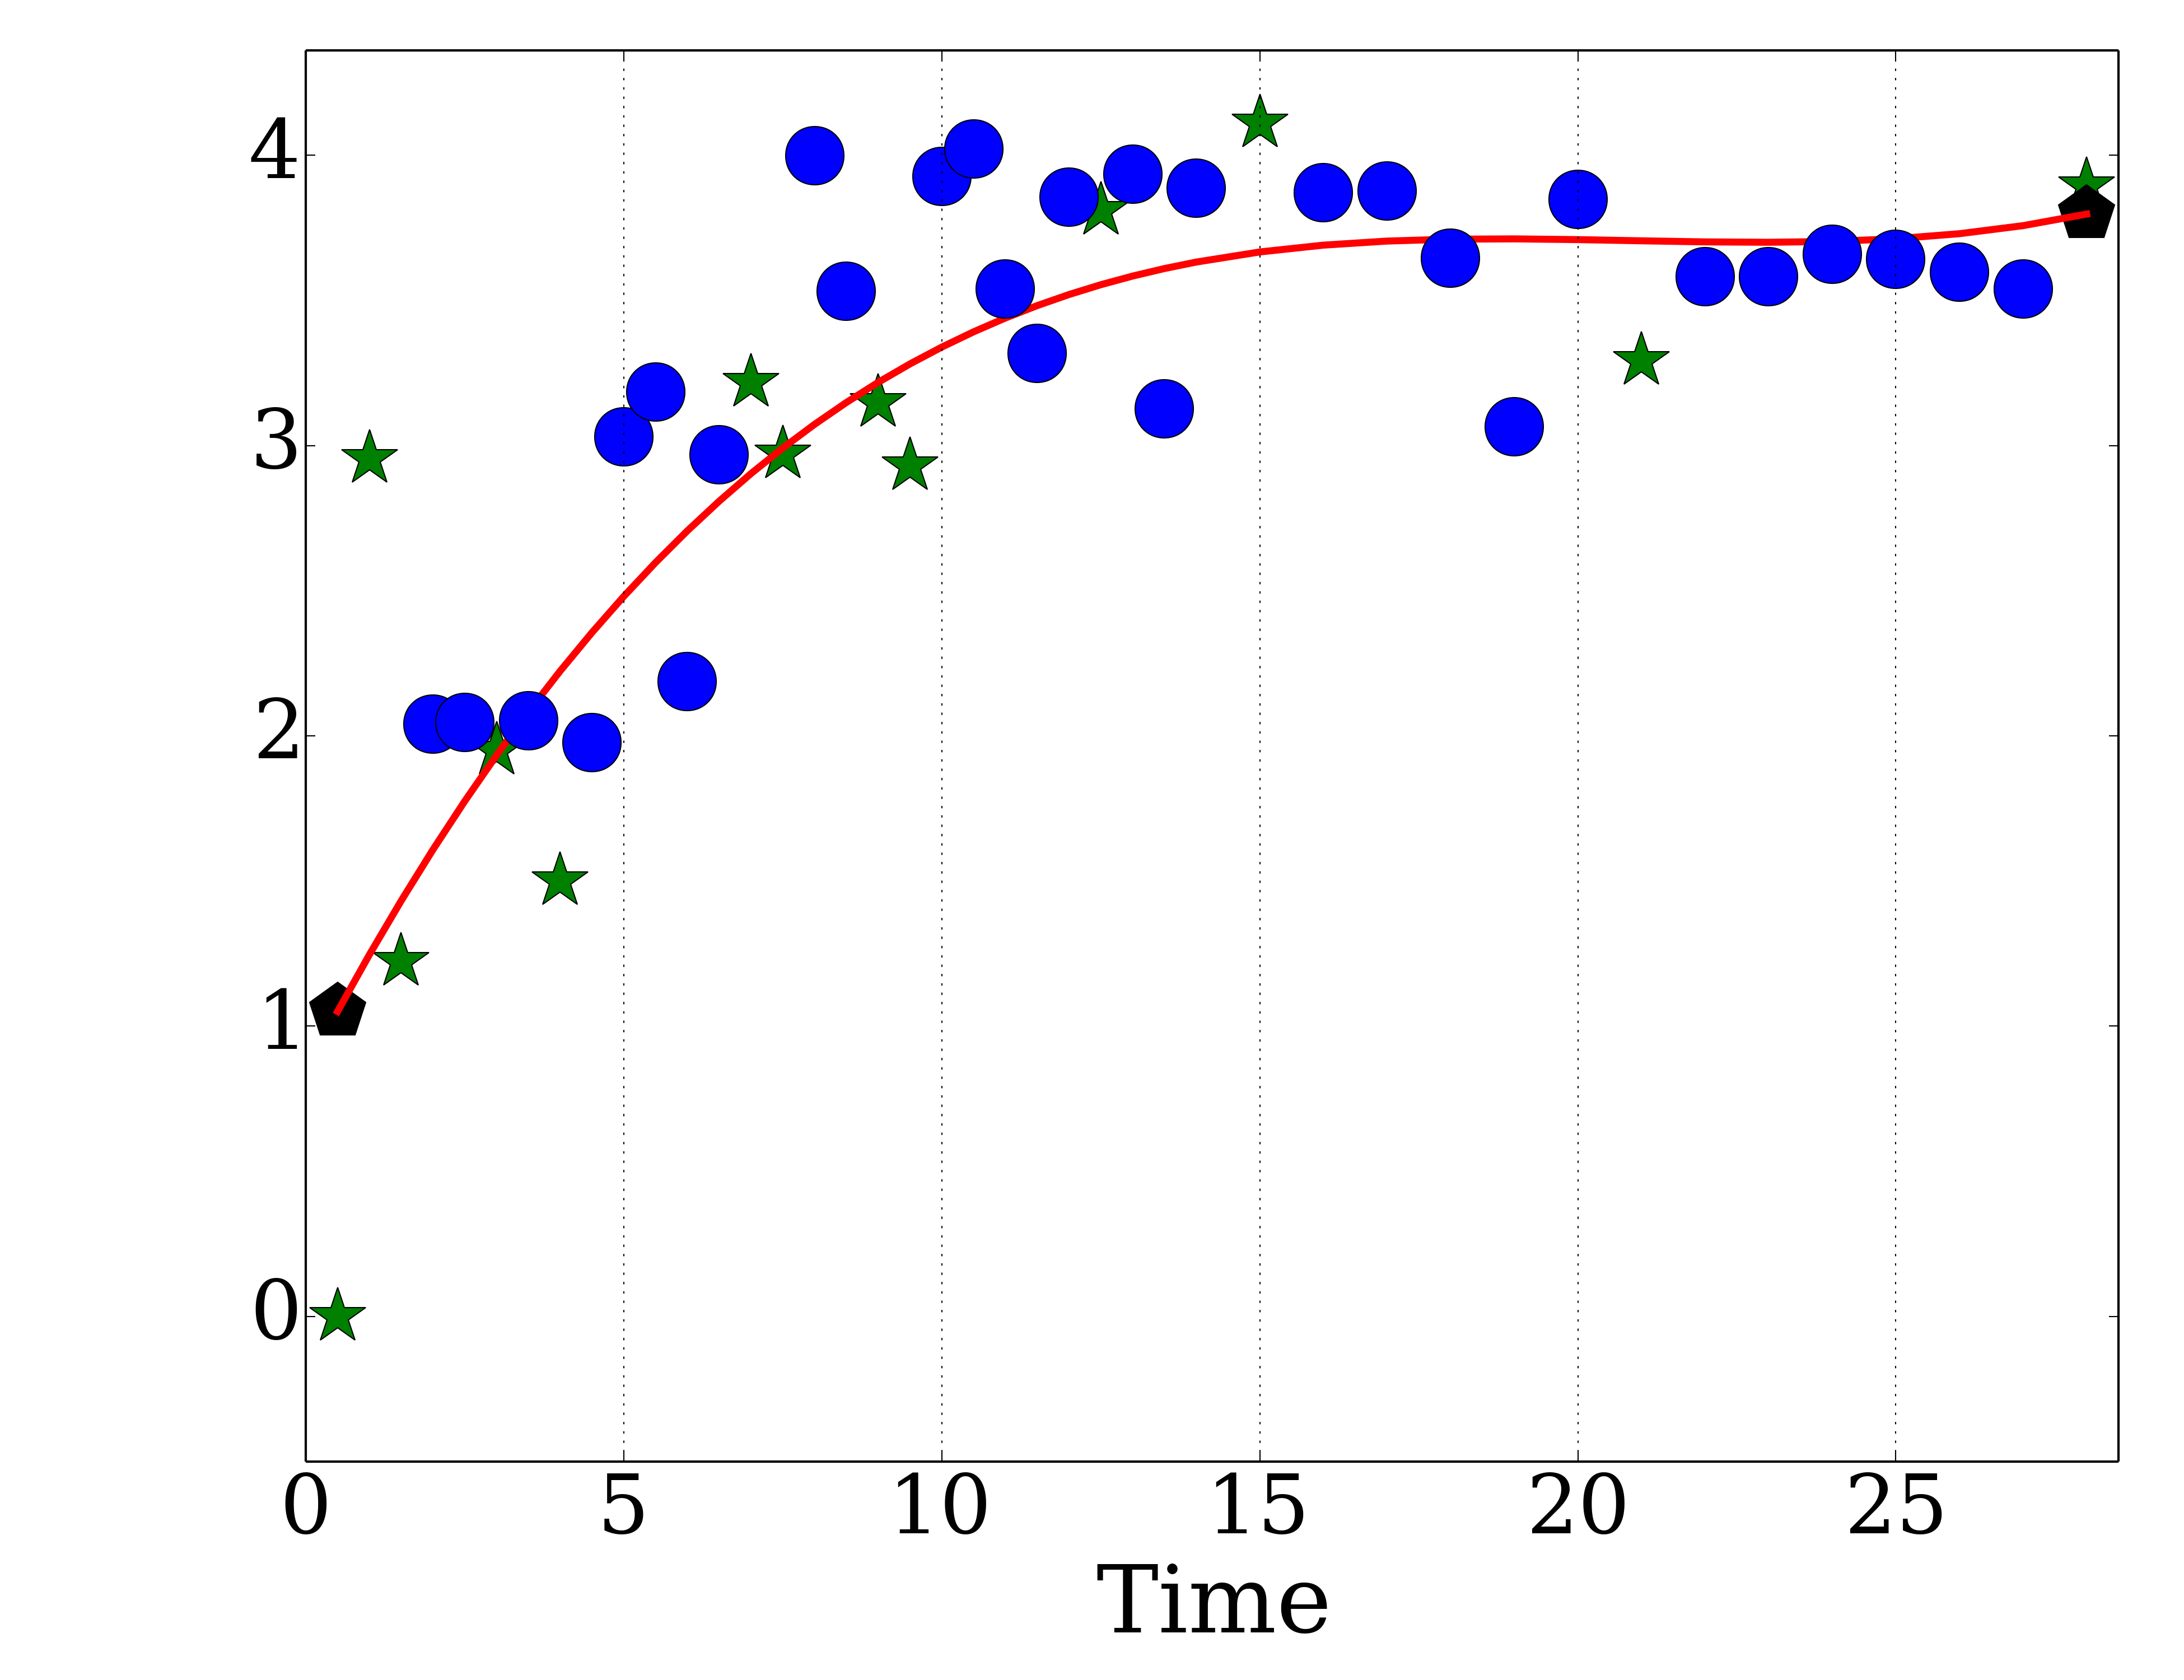
\includegraphics[scale=0.15]{{../mirnadata/splineplots13/uni/mmu-miR-100_13}.png}}
\hfill
\subfloat[mmu-miR-136]{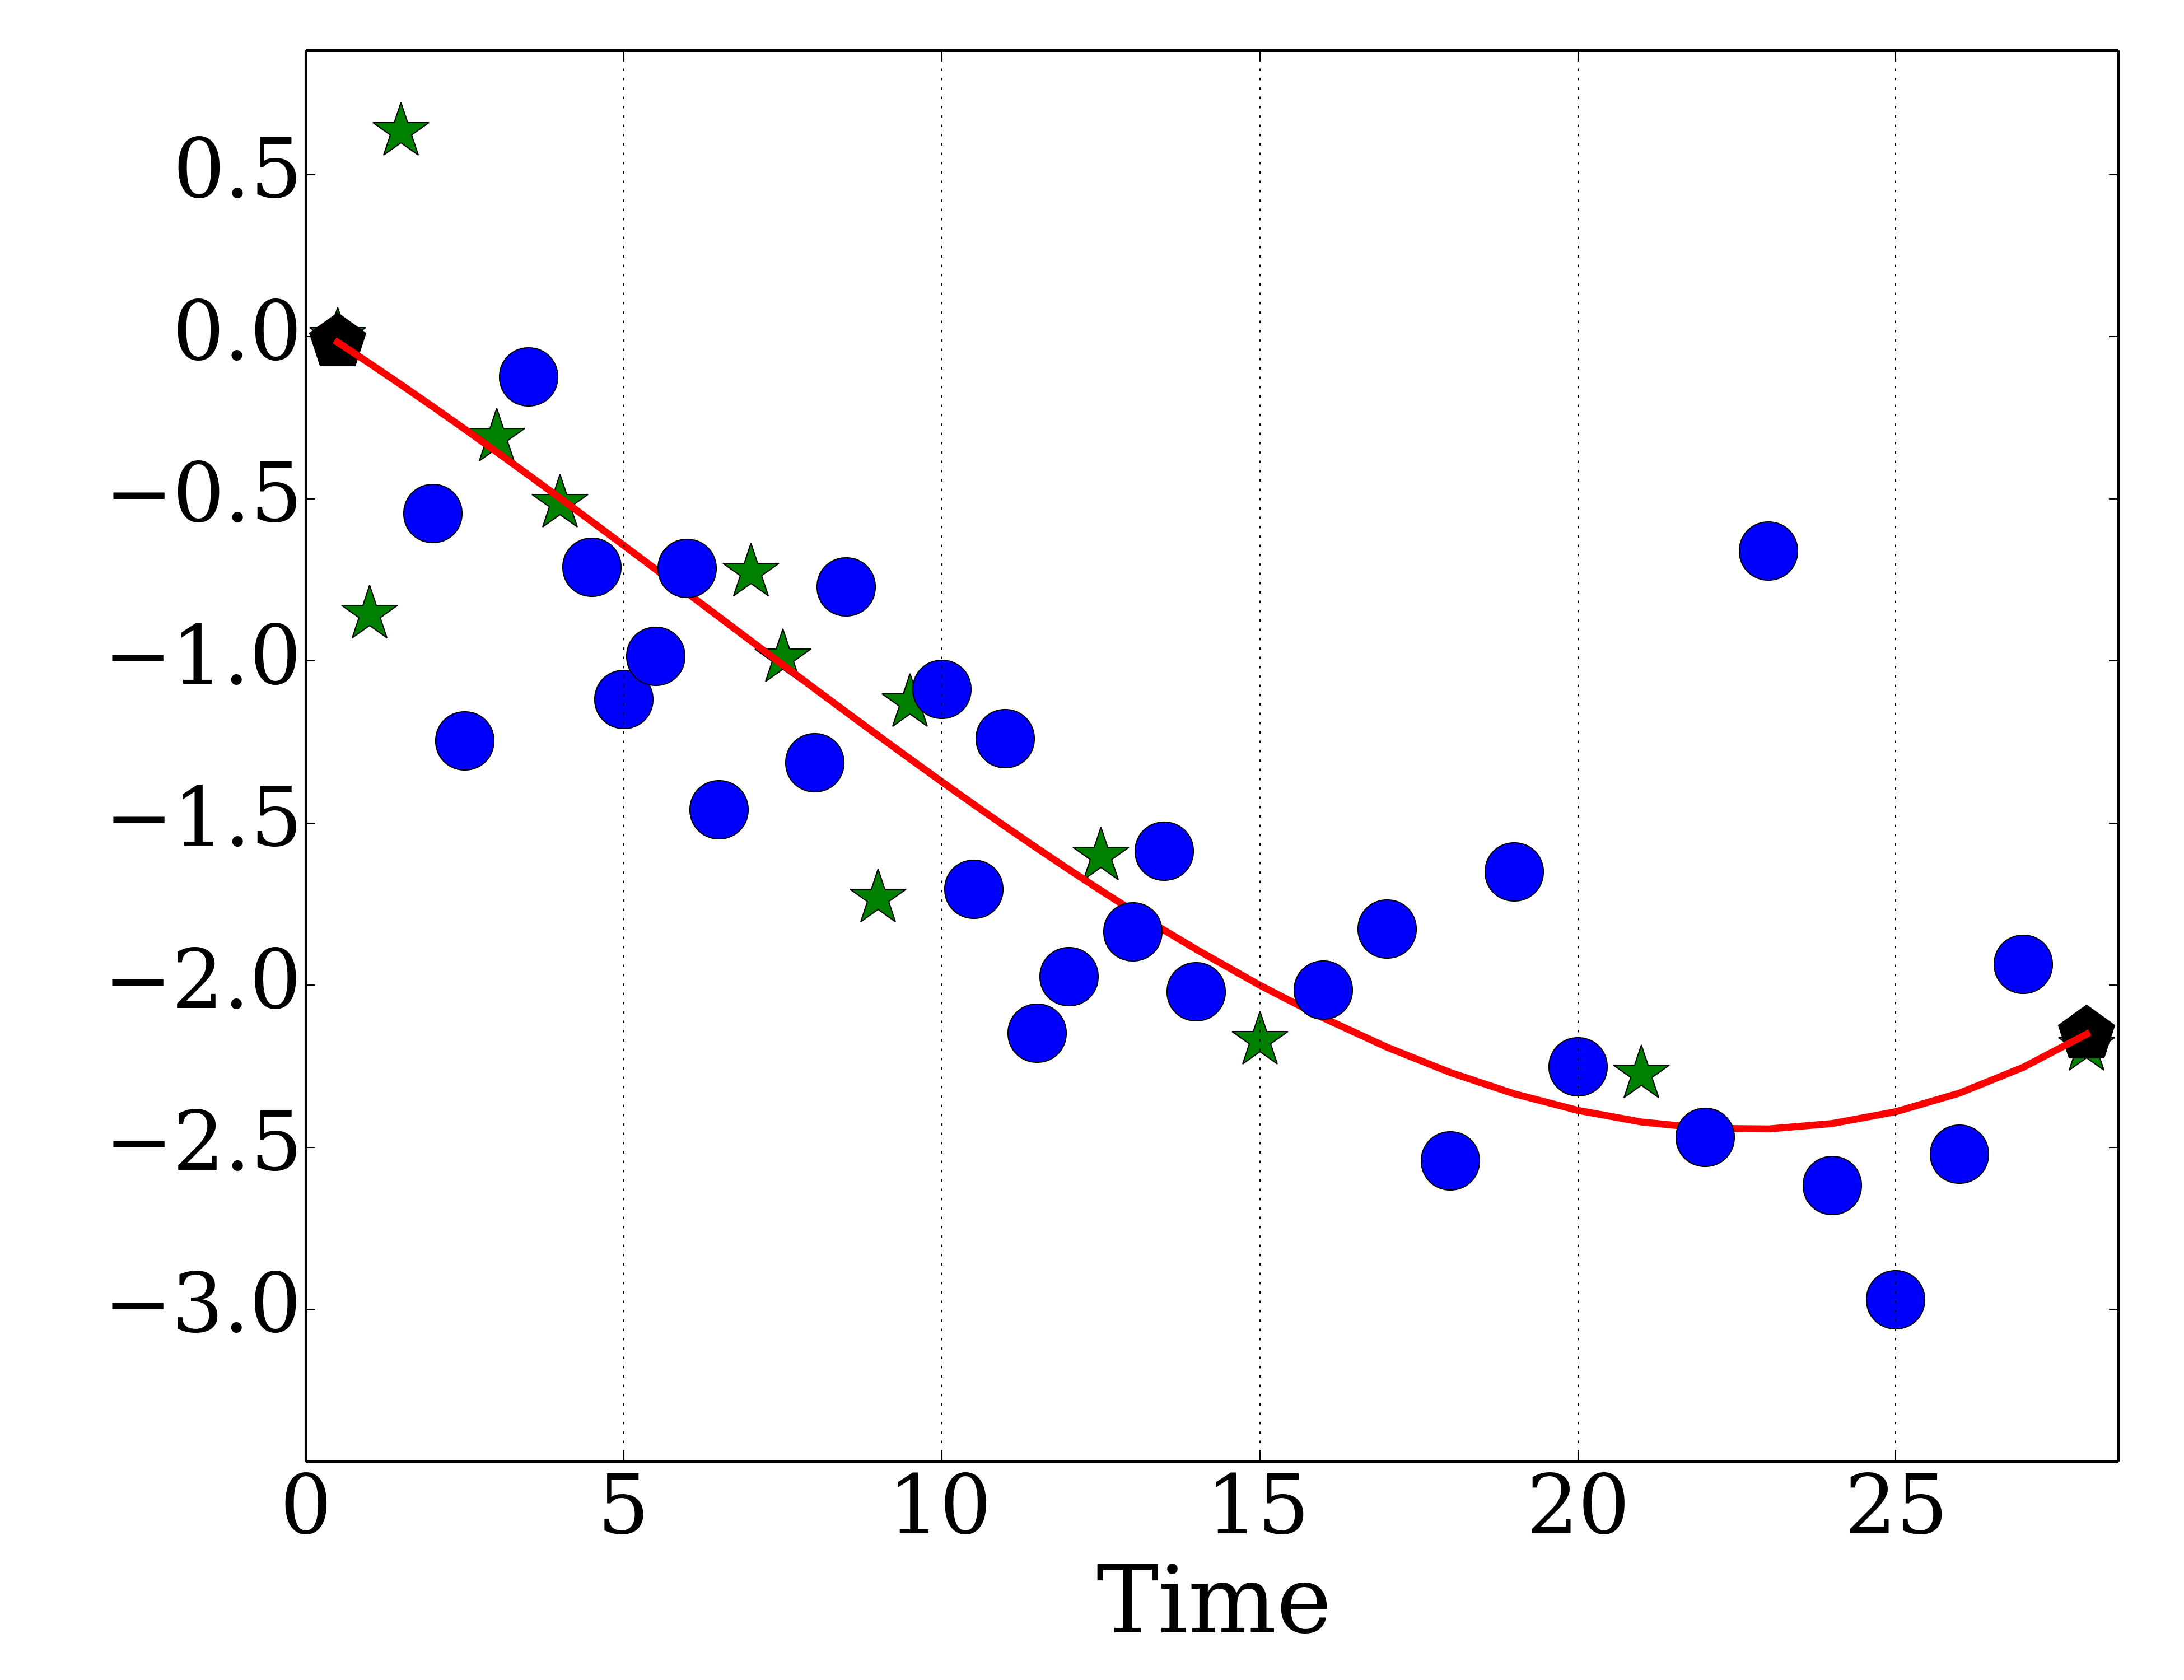
\includegraphics[scale=0.15]{{../mirnadata/splineplots13/uni/mmu-miR-136_13}.png}}
\\
\centering
\hfill
\subfloat[mmu-miR-152]{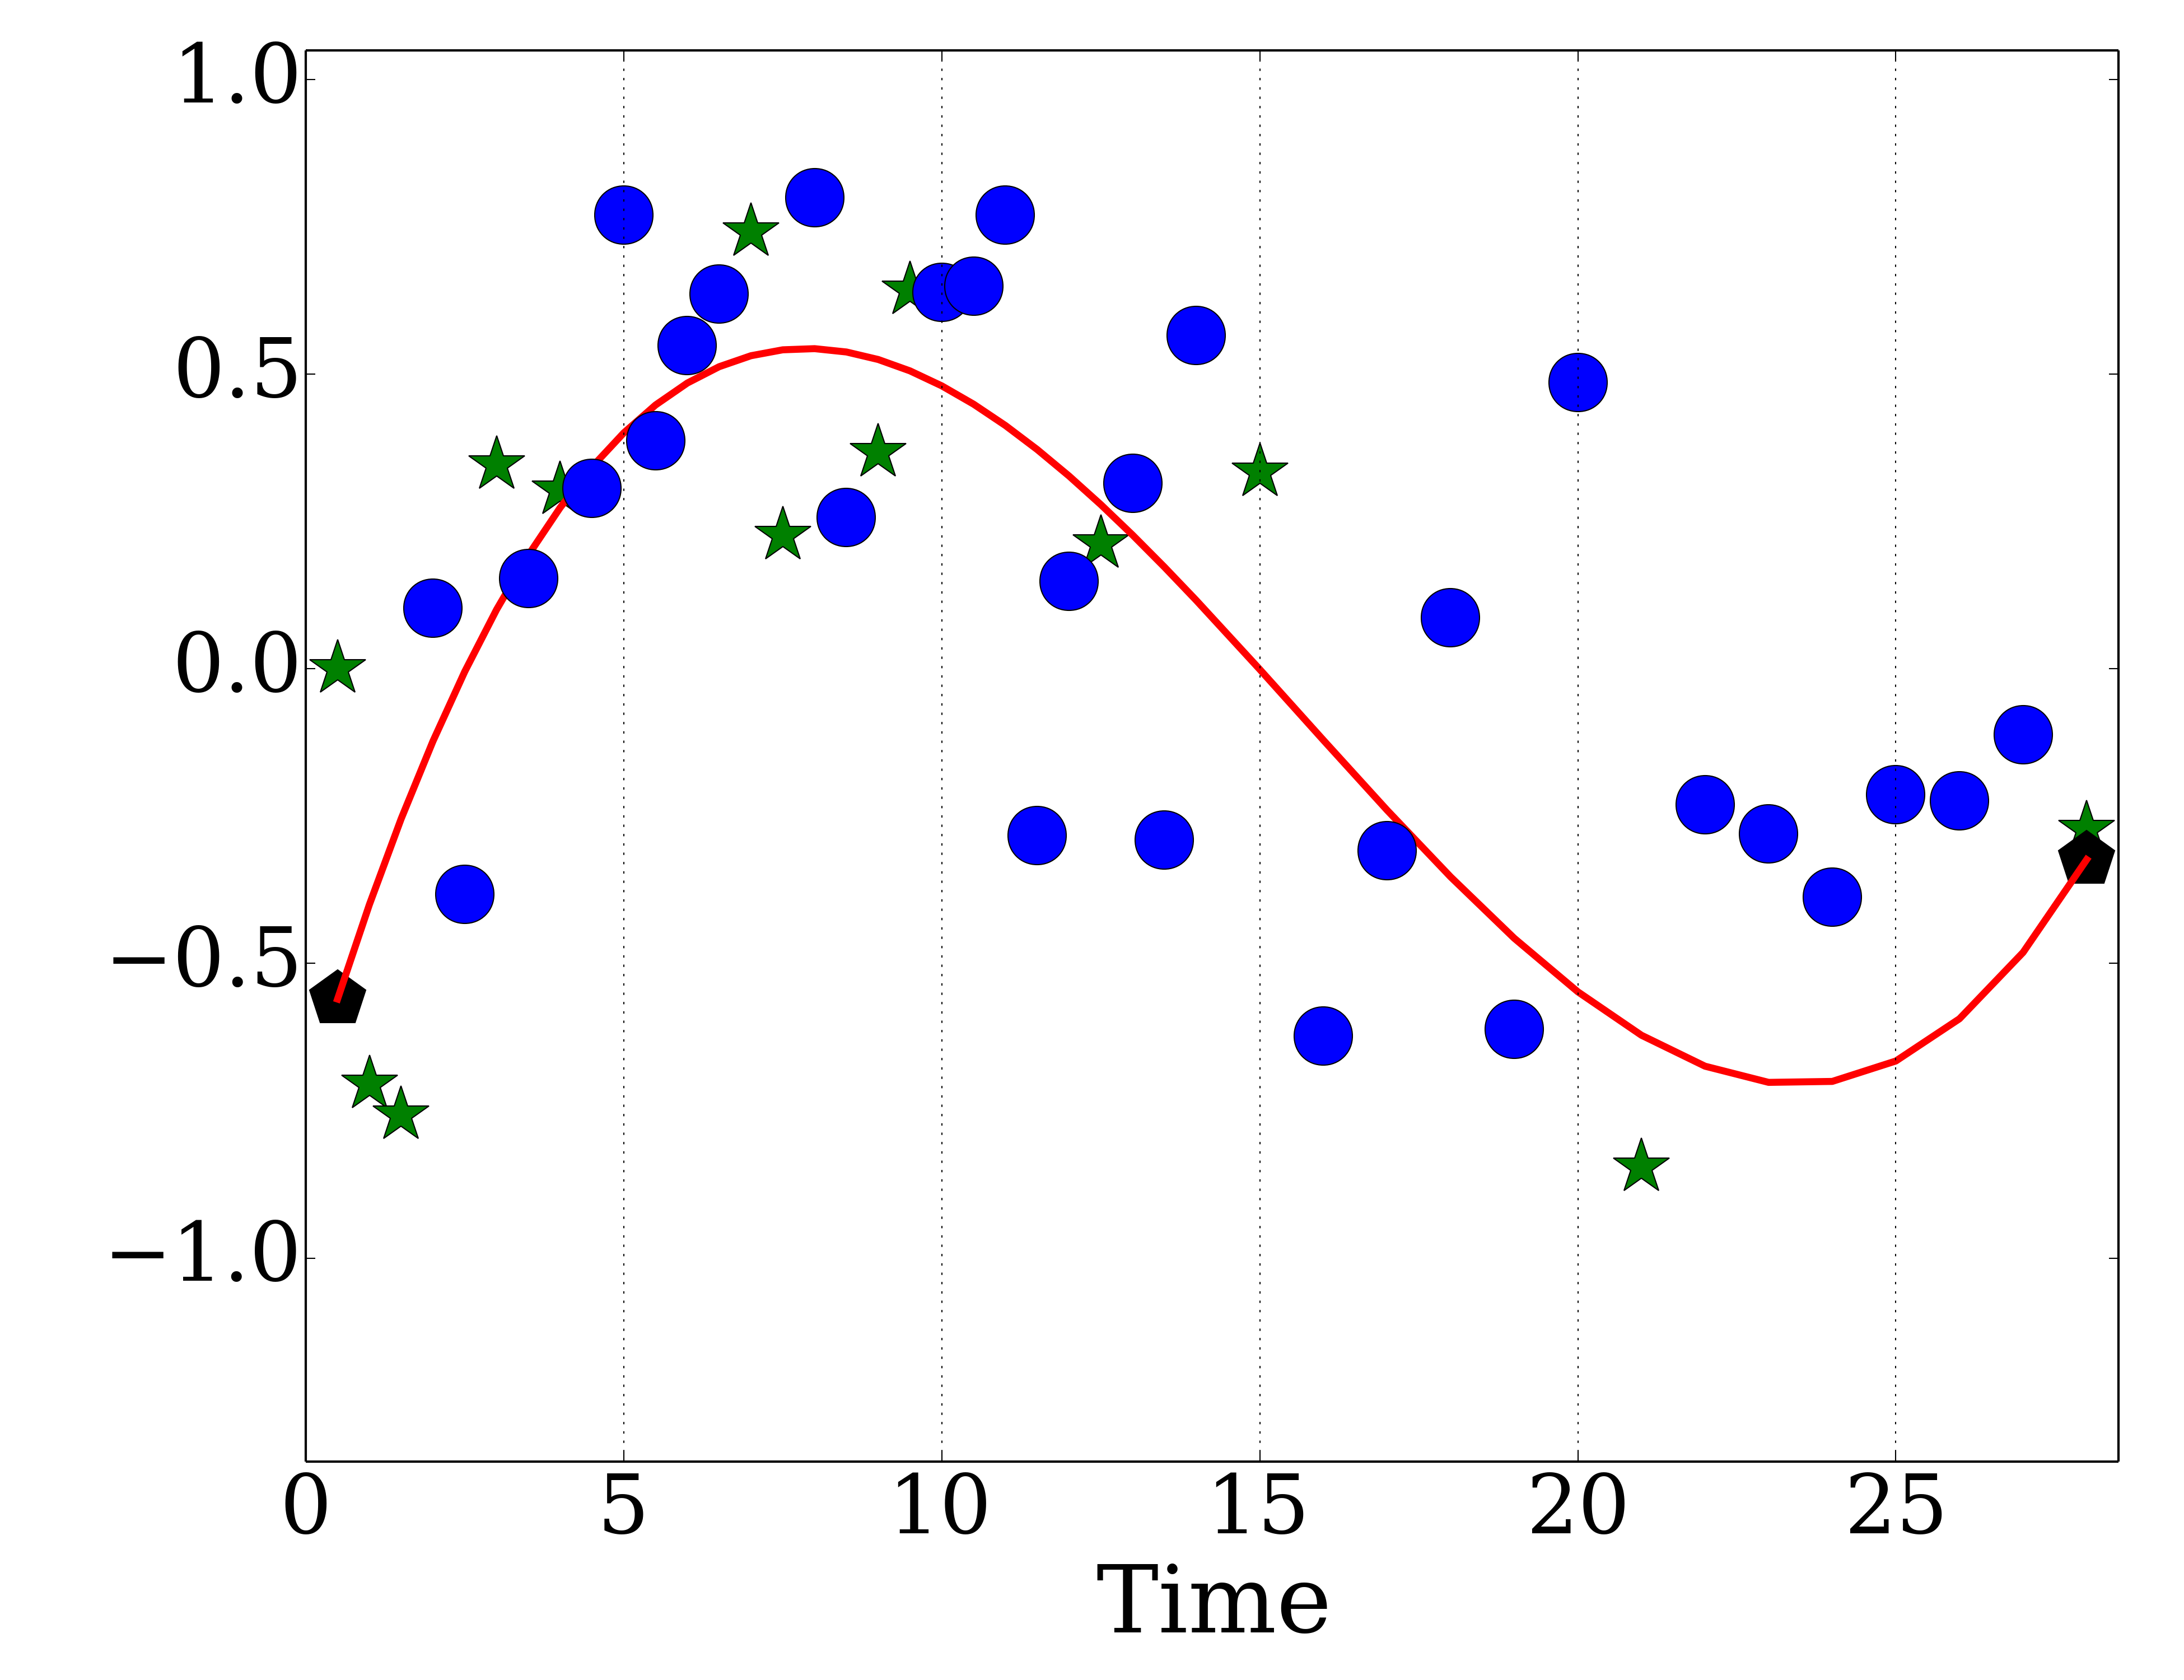
\includegraphics[scale=0.15]{{../mirnadata/splineplots13/uni/mmu-miR-152_13}.png}}
\hfill
\subfloat[mmu-miR-219]{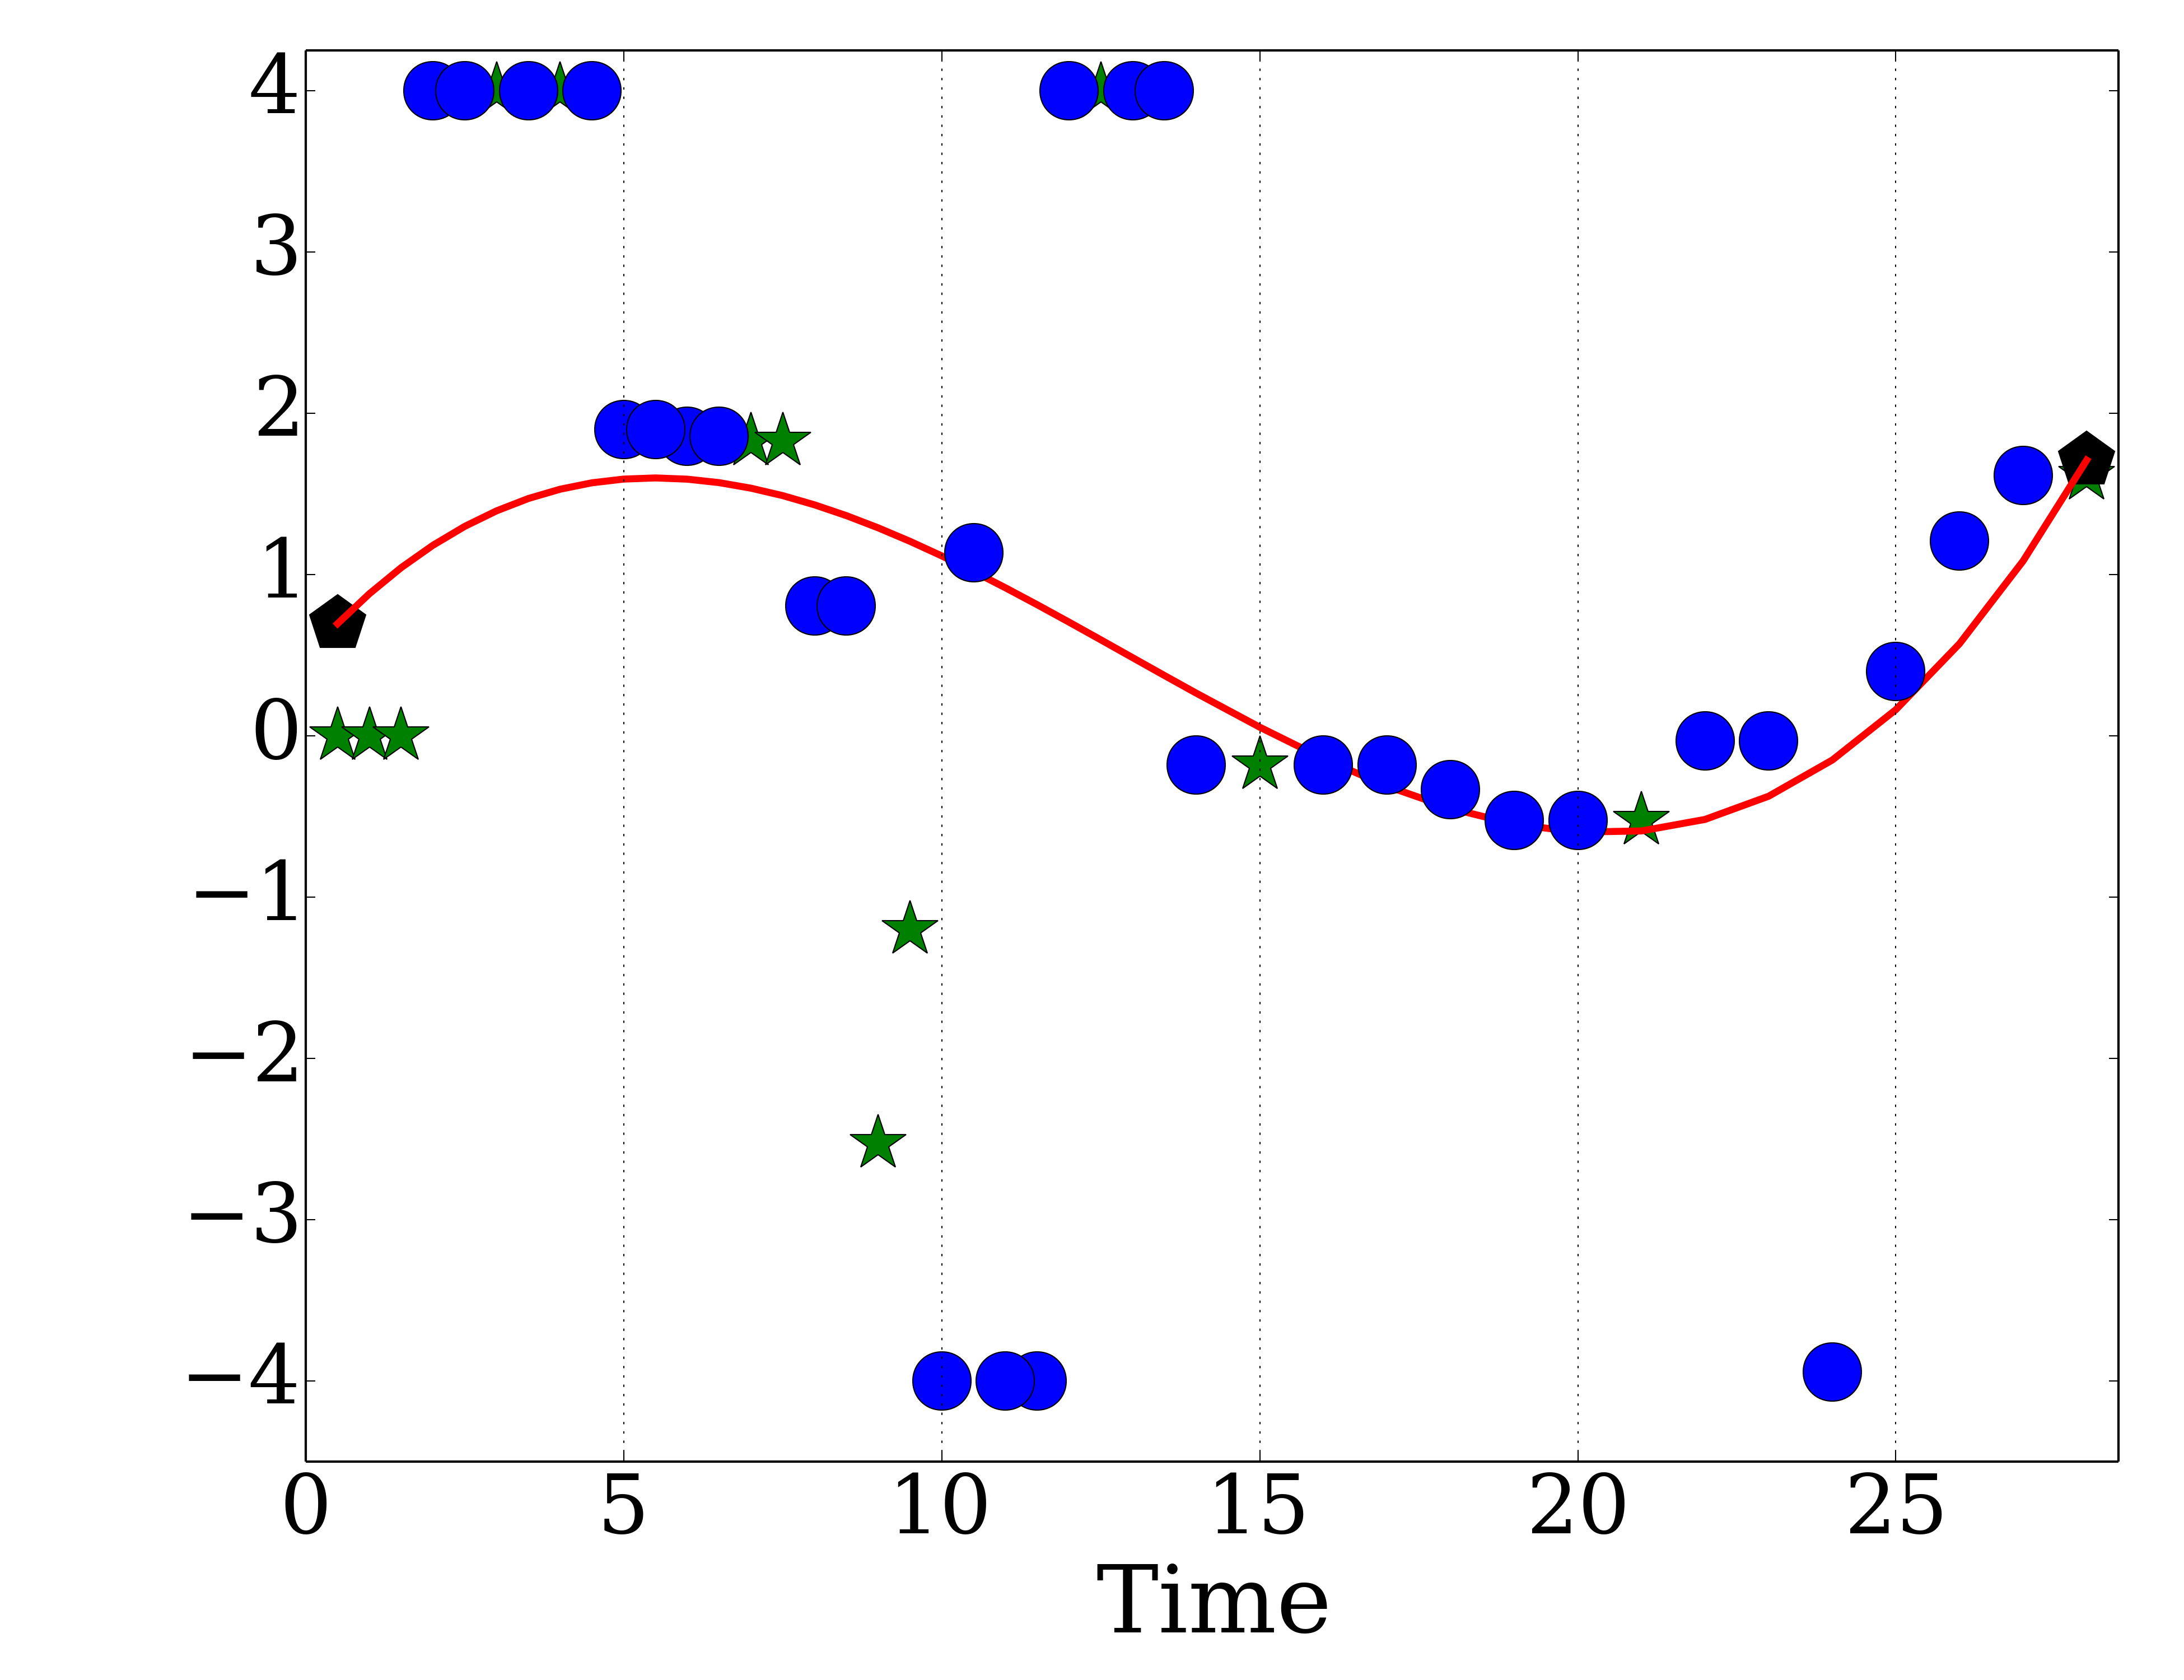
\includegraphics[scale=0.15]{{../mirnadata/splineplots13/uni/mmu-miR-219_13}.png}}
\end{minipage}
\caption{Predicted expression profiles of different miRNAs}
\label{fig:mirnaplots_spec}
\end{figure}

\subsection{Methylation analysis}

\bibliographystyle{plain}
\bibliography{expressbib}

\end{document}
